\setAuthor{Hannes Kuslap}
\setRound{lahtine}
\setYear{2020}
\setNumber{G 2}
\setDifficulty{2}
\setTopic{TODO}

\prob{Ruut fookuses}
Konstrueerige ruudu $ABCD$ tippude ja külgede kujutised kumerläätses, kui on teada, et
	ruudu keskpunkt $F$ on fookuses ja läätse fookuskaugus on võrdne ruudu
	küljepikkusega ($|AB|=|OF|$, kus $O$ on läätse optiline keskpunkt).
	\begin{figure}[h]
		\centering
		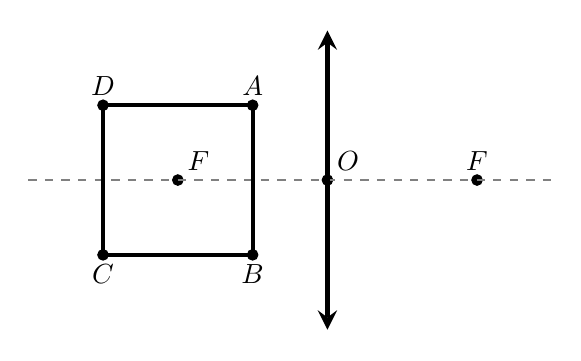
\begin{tikzpicture}[scale=0.95]
			\filldraw[black] (-2,0) circle (2pt) node[anchor=south west] {$F$};
			\filldraw[black] (2,0) circle (2pt) node[anchor=south] {$F$};
			\filldraw[black] (0,0) circle (2pt) node[anchor=south west] {$O$};
			\filldraw[black] (-1,1) circle (2pt) node[anchor=south] {$A$};
			\filldraw[black] (-1,-1) circle (2pt) node[anchor=north] {$B$};
			\filldraw[black] (-3,-1) circle (2pt) node[anchor=north] {$C$};
			\filldraw[black] (-3,1) circle (2pt) node[anchor=south] {$D$};
			\draw[gray] [dashed,-] (-4,0) -- (3,0);
			\draw[black, line width=1.5pt] (-1,1) -- (-1,-1);
			\draw[black, line width=1.5pt] (-1,-1) -- (-3,-1);
			\draw[black, line width=1.5pt] (-3,-1) -- (-3,1);
			\draw[black, line width=1.5pt] (-3,1) -- (-1,1);
			\draw[line width=2pt,>=stealth, <->] (0,-2) -- (0,2);
		\end{tikzpicture}
	\end{figure}
	
	
	\vspace{-10pt}
	
\hint

\solu
\begin{figure}[H]
	\centering
	\resizebox{\linewidth}{!}{%
		\begin{tikzpicture}[scale=1]
			\filldraw[black] (-2,0) circle (2pt) node[anchor=south west] {$F$};
			\filldraw[black] (2,0) circle (2pt) node[anchor=south] {$F$};
			\filldraw[black] (0,0) circle (2pt) node[anchor=south west] {$O$};
			\filldraw[black] (-1,1) circle (2pt) node[anchor=south] {$A$};
			\filldraw[black] (-1,-1) circle (2pt) node[anchor=north] {$B$};
			\filldraw[black] (-3,-1) circle (2pt) node[anchor=north] {$C$};
			\filldraw[black] (-3,1) circle (2pt) node[anchor=south] {$D$};
			\draw[gray] [dashed,-] (-5,0) -- (10,0);
			\draw[black, line width=1.5pt] (-1,1) -- (-1,-1);
			\draw[black, line width=1.5pt] (-1,-1) -- (-3,-1);
			\draw[black, line width=1.5pt] (-3,-1) -- (-3,1);
			\draw[black, line width=1.5pt] (-3,1) -- (-1,1);
			
			\draw[line width=2pt,>=stealth, <->] (0,-2) -- (0,2);
			
			\draw [dotted] (-1,1) -- (0,1);
			\draw [dotted] (-1,-1) -- (0,-1);
			\draw [dotted] (-5,-3.5) -- (10,4);
			\draw [dotted] (-5,3.5) -- (10,-4);
			
			\draw [dotted](0,0) -- (-5,5);
			\draw [dotted](0,0) -- (-5,-5);
			\draw [dotted](-3,-1) -- (10, 3.3333);
			\draw [dotted](-3,1) -- (10,-3.3333);
			
			\filldraw[black] (-2,2) circle (2pt) node[anchor=south] {$A'$};
			\filldraw[black] (-2,-2) circle (2pt) node[anchor=north] {$B'$};
			\filldraw[black] (6,2) circle (2pt) node[anchor=north west] {$C'$};
			\filldraw[black] (6,-2) circle (2pt) node[anchor=south west] {$D'$};
			
			\draw[black,line width=1pt] (-2, 2) -- (-2,  -2);
			\draw[black,line width=1pt] (-2, 2) -- (-5, 3.5);
			\draw[black,line width=1pt] (-2,-2) -- (-5,-3.5);
			\draw[black,line width=1pt] ( 6, 2) -- ( 6,  -2);
			\draw[black,line width=1pt] ( 6, 2) -- ( 9,  3.5);
			\draw[black,line width=1pt] ( 6,-2) -- ( 9, -3.5);
			\draw[black,line width=1pt,dashed] ( 9,-3.5) -- (10, -4);
			\draw[black,line width=1pt,dashed] ( 9, 3.5) -- (10,  4);
			\draw[black,line width=1pt,dashed] (-5,-3.5) -- (-6, -4);
			\draw[black,line width=1pt,dashed] (-5, 3.5) -- (-6,  4);
			
			\filldraw[black] (-2.6,1) circle (2pt) node[anchor=south] {$K$};
			\filldraw[black] (-1.4,1) circle (2pt) node[anchor=south] {$L$};
			\filldraw[black] (-4.667,3.333) circle (2pt) node[anchor=south] {$L'$};
			\filldraw[black] (8.667,-3.333) circle (2pt) node[anchor=south] {$K'$};
			\draw [dotted](0,0) -- (-4.667,3.333);
			\draw [dotted](-2.6,1) -- (8.667,-3.333);
		\end{tikzpicture}
	}%
\end{figure}
Leiame punktide $A, B, C$ ja $D$ kujutised $A', B', C'$ ja $D'$ läätses eraldi. Ühendame vertikaalsed küljed $A'B'$ ja $C'D'$. Märkame, et punktid $A'$ ja $B'$ on teisel pool läätse kui punktid $C'$ ja $D'$. Seega ei ole lõigu $AD$ kujutis lõik $A'D$. Valime küljel $AD$ abipunktid $K$ ja $L$, mis asuks vastavalt vasakul ja paremal pool fookusest. Seega on külje $AD$ fookusest paremal oleva osa kujutis sirgel $A'L'$ ja fookusest vasakul oleva osa kujutis sirgel $D'K'$. Kuna mistahes $L$ ja $K$ puhul on need fookusele lähemal kui $A$ ja $D$, siis on ka lõigust $AD$ iga punkti kujutis läätsest kaugemal, kui $A'$ ja $D'$.
Analoogselt leiame ka $BC$ kujutise.
\probend